\documentclass[a4paper]{article}
\usepackage[utf8]{inputenc} 	% codificacao de caracteres
\usepackage[T1]{fontenc}    	% codificacao de fontes
\usepackage[portuges]{babel}  	% idioma
\usepackage[table]{xcolor}    	% linhas coloridas alternadamente
\usepackage{graphicx}
\usepackage{multirow}
\usepackage{soulutf8}			% cor de fundo do texto que aceita utf8
\usepackage{makecell}			% mais de uma linha na célula da tabela
\usepackage[pdftex]{hyperref}
\usepackage[font=small,labelfont=bf]{caption} 



% espaçamento paragrafos
\setlength{\parindent}{0em}
%\setlength{\parskip}{2em}
%\renewcommand{\baselinestretch}{1}

%opening
\title{Universidade do Minho}
\author{Grupo 1}
\date{}

\begin{document}



\begin{center}
	
\includegraphics[scale=0.5]{images/um}
\end{center}


\begin{center}
	\vspace{14ex}
	\LARGE
	Departamento de Informática\\	
	\Huge
	Comunicações por Computador\\
	\vspace{7ex}
	\textbf{{
			\LARGE Trabalho Prático nº 3
	}}\\
	\vspace{5ex}
	{\large 
		Serviço de Resolução de Nomes (DNS)\\
		Ano Letivo 2020/2021
	}
	\vspace{6ex}
\end{center}



\textbf{Grupo 1 - PL1}\\

Ana Filipa Pereira		A89589\\
Carolina Santejo		A89500  \\
Raquel Costa			A89464 \\




\newpage

\tableofcontents

\newpage


\section{Questões e Respostas - Parte I }


\subsection{ a)} \textbf{Q: Qual o conteúdo do ficheiro /etc/resolv.conf e para que serve essa informação?} \par

\begin{center}
	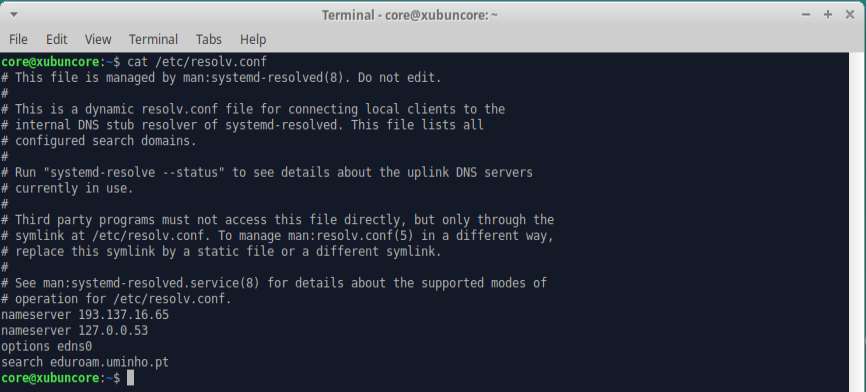
\includegraphics[scale=0.5]{images/1a}
	\captionof{figure}{Conteúdo do ficheiro resolv.conf}
\end{center}


Este ficheiro contém os servidores DNS por defeito da maquina, estabelecidos pelo administrador de rede, que serão os responsáveis por fazer a resolução de nomes e IPs.

\subsection{ b)} \textbf{Q: Os servidores www.uminho.pt.e  www.ubuntu.com. têm endereços IPv6?  Se sim, quais?} \par

\begin{center}
	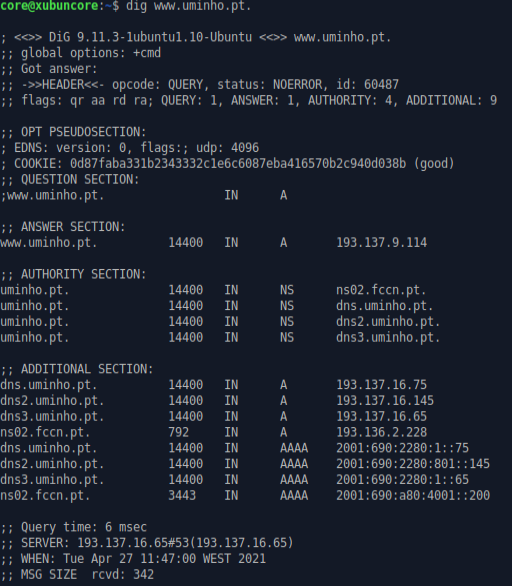
\includegraphics[scale=0.5]{images/1bUminho}
	\captionof{figure}{ Comando dig para www.uminho.pt.} 
\end{center}

\begin{center}
	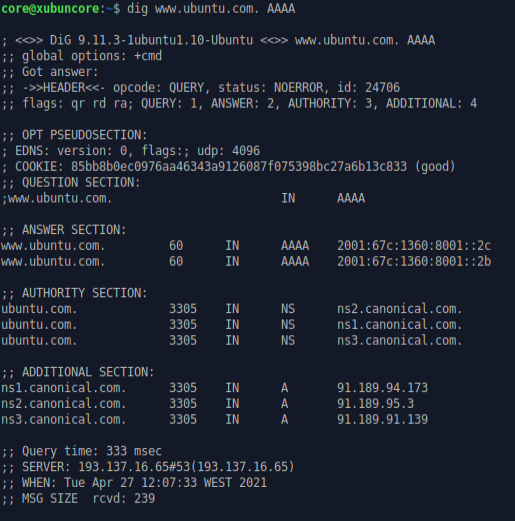
\includegraphics[scale=0.5]{images/1bUbuntu}
	\captionof{figure}{Comando dig para www.ubuntu.com.} 
\end{center}

Para verificar a existência de endereços IPv6 num servidor foi necessário procurar a ocorrencia do identificador AAAA nas informações do comando dig. Sendo assim, podemos verificar que para os servidores www.uminho.pt. identifica-se que os 4 existentes possuem endereços IPv6, sendo eles:\\
2001:690:2280:1::75\\
2001:690:2280:801::145\\
2001:690:2280:1::65\\
2001:690:a80:4001::200\\
Para o caso do www.ubuntu.com. também se verifica a existencia de 2 endereços IPv6:\\
2001:67c:1360:8001::2c\\
2001:67c:1360:8001::2b\\

\subsection{ c)} \textbf{Q: Quais os servidores de nomes definidos para os domínios: “sapo.pt.”, “pt.” e “.”?} \par

Para identificar os servidores de nomes de um domínio foi necessário utilizar o comando dig com a flag NS. Para cada um dos domínios “sapo.pt.”, “pt.” e “.” estão identificados os respetivos servidores na secção de resposta.

\begin{center}
	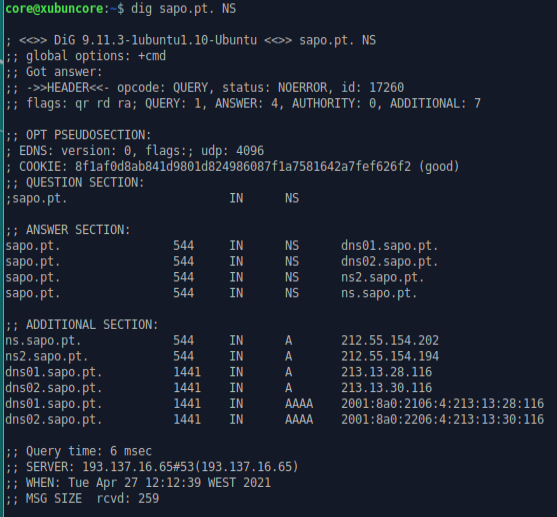
\includegraphics[scale=0.6]{images/1cSapo}
	\captionof{figure}{Comando dig para sapo.pt.}
\end{center}

\begin{center}
	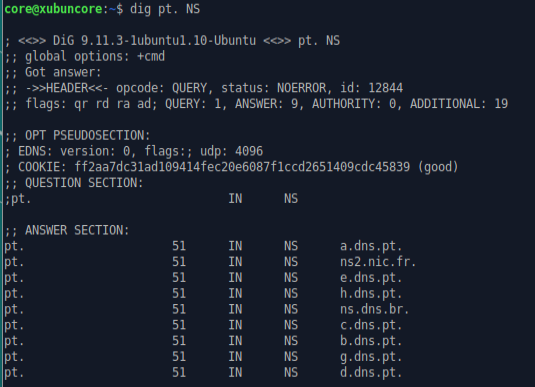
\includegraphics[scale=0.6]{images/1cPt}
	\captionof{figure}{Comando dig para pt.} 
\end{center}

\begin{center}
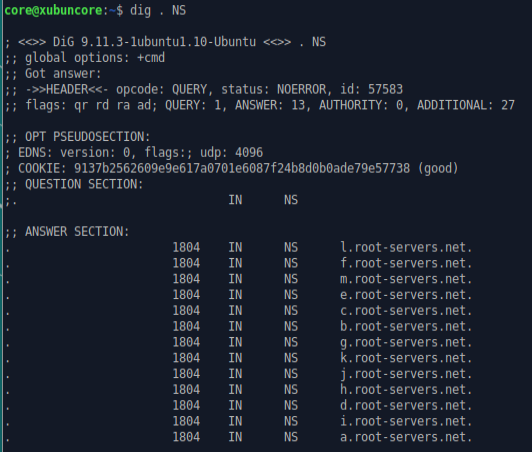
\includegraphics[scale=0.6]{images/1cRoot}
\captionof{figure}{ Comando dig para .}
\end{center}

\subsection{ d)} \textbf{Q: Existe o domínio open.money.? Será que open.money. é um host ou um domínio?} \par

Sim, existe o domínio open.money. e é um host porque possui um endereço IP como pode verificar na figura abaixo.

\begin{center}
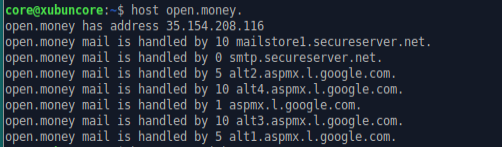
\includegraphics[scale=1]{images/1d}
\captionof{figure}{ Comando host para open.money.} 
\end{center}

\subsection{ e)} \textbf{Q: Qual  é  o  servidor DNS primário  definido para  o  domínio un.org.? Este  servidor  primário  (master)  aceita  queries  recursivas? Porquê?} \par

DNS primário: ns1.un.org.\\
Este servidor aceita queries recursivas uma vez que na resposta ao comando dig está presente 'ra' que significa \textit{recursion available}.

\begin{center}

\includegraphics[scale=1]{images/1eHost}
\captionof{figure}{Comando host para un.org.} 
\end{center}


\begin{center}
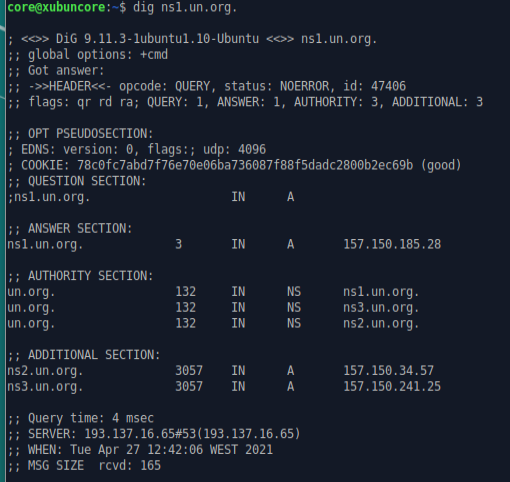
\includegraphics[scale=1]{images/1eDig}
\captionof{figure}{Comando dig para un.org.} 
\end{center}

\newpage

\subsection{ f)} \textbf{ Q: Obtenha uma resposta “autoritativa” para a questão anterior.}
\qquad Para obter uma resposta autoritativa foi necessário a utilização de uma query NS. De seguida realizou-se uma query dig a um dos servidores listados.  OU NÃO FOI POSSIVEL OBTER UMA RESPOSTA AUTORITATIVA "AUTHORITY 0"	\par
\qquad TIRAR DUVIDA NA AULA	

\begin{center}
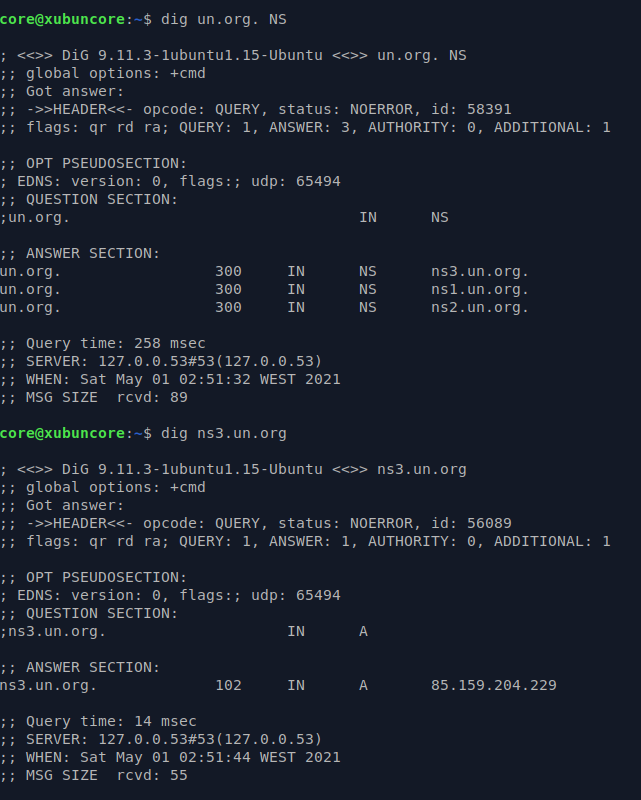
\includegraphics[scale=0.5]{images/authority}
\captionof{figure}{...} 
\end{center}

\newpage

\subsection{ g)} \textbf{ Q: Onde são entregues as  mensagens de correio eletrónico dirigidas a presidency@eu.eu ou presidencia@2021portugal.eu?}\par
\qquad Para verificar onde são entregues as mensagens de correio eletrónico utilizamos queries MX, isto é, "Mail Exchanger". Deste modo foi possível concluir o seguinte :\par
\qquad >> No caso do eu.eu., as mensagens são entregues no servidor mxg.eu.mpssec.net.

\begin{center}
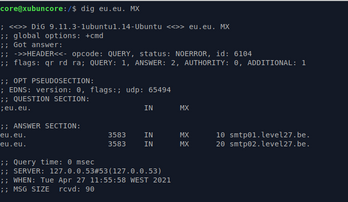
\includegraphics[scale=0.75]{images/eu.eu}
\captionof{figure}{Comando dig para eu.eu.} 
\end{center}


\qquad >>Para 2021portugal.eu., as mensagens são entregues nos servidores smtp01.level27.be. e smtp02.level27.be.

\begin{center}
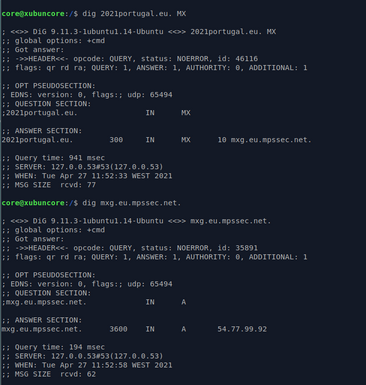
\includegraphics[scale=0.7]{images/2021portugal.eu}
\captionof{figure}{Comando dig para 2021portugal.eu.} 
\end{center}

\begin{center}
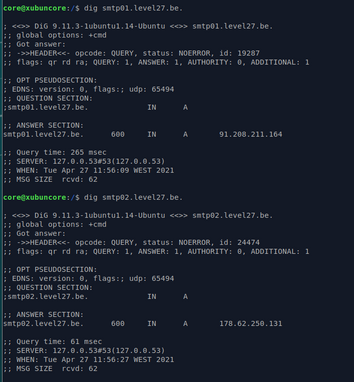
\includegraphics[scale=0.7]{images/smt01-02}
\captionof{figure}{Comando dig para servidores smtp01.level27.be. e  smtp02.level27.be.} 
\end{center}

\subsection{ h)} \textbf{ Q: Que informação é possível obter, via DNS, acerca de gov.pt?}



\subsection{ i)} \textbf{ Consegue interrogar o DNS sobre o endereço IPv6 2001:690:2080:8005::38 usando algum dos clientes DNS? Que informação consegue obter? Supondo que teve problemas com esse endereço, consegue obter um contacto do responsável por esse IPv6?}

\newpage

\subsection{ j)} \textbf{ Os secundários usam um mecanismo designado por “Transferência de zona” para se atualizarem automaticamente a partir do primário, usando os parâmetros definidos no Record do tipo SOA do domínio. Descreve sucintamente esse mecanismo com base num exemplo concreto (ex: di.uminho.pt ou o domínio cc.pt que vai ser criado na topologia virtual).}\par

\qquad O mecanismo de "Transferência de zona" permite replicar uma porção ou a totalidade da base de 
dados DNS do servidor primário para o secundário. Além disso, esta transferência é realizada sempre sobre TCP, assumindo a forma de uma transação cliente-servidor, onde o cliente que solicita a transferência trata-se de um servidor "slave" ou secundário.\par
\qquad  Por exemplo, analisando os parâmetros definidos e os campos no Record do tipo SOA do domínio di.uminho.pt, é possível observar o campo SERIAL, que representa o número de série da zona em questão.  Caso um servidor secundário observar um incremento neste número então irá assumir que esta zona já foi atualizada e irá inicializar a "transferência de zona", caso contrário, isto é, caso o número de série seja o mesmo ou inferior então a transferência não irá ocorrer, uma vez que o servidor secundário que está a solicitar o pedido contém uma versão da base de dados igual ou mais atual.\par
\qquad Note-se também na existência de outros campos no Record do SOA que contém valores temporais, tais como, o refresh, retry, expire e minimum.
	
\begin{center}
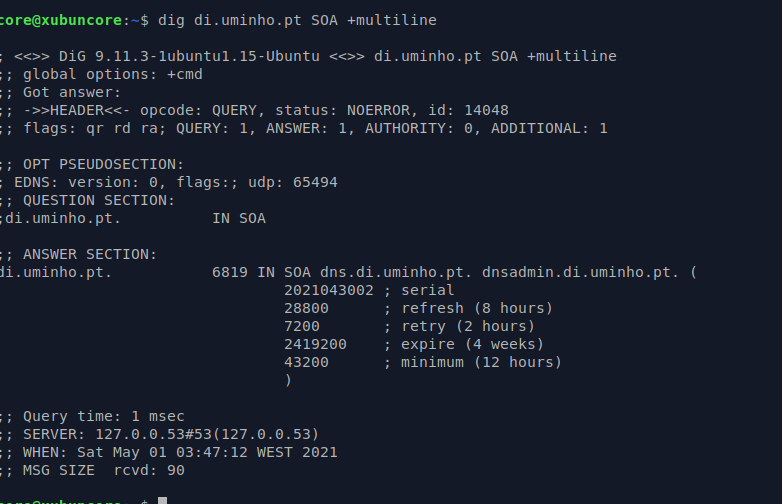
\includegraphics[scale=0.5]{images/SOA}
\captionof{figure}{Comando dig di.uminho.pt. SOA } 
\end{center}

\newpage

\section{Parte II }

\end{document}